\documentclass[11pt]{article}

\usepackage[utf8]{inputenc}
\usepackage[T1]{fontenc}
\usepackage[english]{babel}

\usepackage[letterpaper,top=2cm,bottom=2cm,left=3cm,right=3cm,marginparwidth=1.75cm]{geometry}

\usepackage{amsmath}
\usepackage{graphicx}
\usepackage{url}
\usepackage[colorlinks=true, allcolors=blue]{hyperref}

\title{CrimKG-RU: A Legal Knowledge Graph over Russian Criminal Court Decisions}
\author{
  Daria Ryzhikova \\ ITMO University \\ \texttt{dasha200212345@mail.ru}
  \and
  Sergey Kovalchuk \\ ITMO University \\ \texttt{sergey.kovalchuk@itmo.ru}
  \and
  Oleg Metsker \\ Sirius University of Science and Technology \\ \texttt{oleg.metsker@example.com}
}

\date{June 2026}

\begin{document}
\typeout{*** THIS IS THE MAIN FILE ***}
\maketitle

\begin{abstract}
Analyzing criminal court decisions at scale requires structured representations that go beyond keyword search and flat document retrieval. In the Russian Federation, courts publish large volumes of criminal decisions in machine-readable form, yet this corpus remains under-exploited by legal NLP despite its size and regular publication practices. This paper presents a pipeline for constructing a legal knowledge graph over Russian criminal court decisions, combining rule-based named entity recognition (NER) for Criminal Code article references with a hybrid NER module for persons, and storing the resulting structured data in a Neo4j property graph database. The pipeline processes raw JSON-encoded court decisions, extracts article references using a set of hand-crafted regular expressions covering the major surface forms of Russian Criminal Code citations, and identifies case participants using the Natasha NLP toolkit augmented with a regex fallback for abbreviated name forms. Extracted entities and relations are loaded into Neo4j, producing a corpus-scale graph with 69{,}035 nodes and 399{,}551 relationships. The regex-based article extractor achieves precision 1.000, recall 0.955, and F1 0.977 on a manually annotated evaluation set at the article-number level—the matching criterion that corresponds directly to the graph schema—reflecting the deterministic and highly regular nature of Criminal Code citation syntax in Russian judicial text. Person NER achieves F1 0.961 with perfect recall on a 50-mention annotated subset. The system is complemented by a Streamlit-based demonstration interface supporting case search, document card inspection, local graph visualization, and graph-level descriptive statistics. The main contribution is an open prototype pipeline for legal entity extraction and knowledge graph construction over Russian criminal case materials, together with a transparent multi-level evaluation framework that explicitly separates graph-node linkage from strict span-level extraction and discusses the limitations and ethical constraints of this deterministic, jurisdiction-specific setup.
\end{abstract}

\section{Introduction}

Court decisions are among the most information-dense legal documents produced by any judicial system. A single criminal judgment may reference multiple statutory provisions, name several procedural participants, describe a sequence of events, record a court and its jurisdiction, and specify a penalty---all within a single text of several thousand words. At the scale of a national judicial system, many thousands of such decisions are published each year and made available in electronic form, yet they remain largely unstructured, limiting systematic analysis. Researchers, legal practitioners, and policy analysts who wish to study sentencing patterns, the distribution of criminal charges across regions, or the exposure of individual courts to particular types of offences currently have no structured resource to query.

In the Russian Federation, criminal court decisions are published on official judicial portals in a relatively standardized format, with a strong emphasis on citing provisions of the Criminal Code and anonymizing personal data. This combination of extensive coverage, formalized citation practice, and consistent anonymization makes Russian criminal cases an attractive but underexplored target for legal NLP and knowledge graph construction. Unlike jurisdictions where only a narrow subset of decisions is available, Russian criminal judgments often include detailed factual narratives and explicit statutory references.

Knowledge graphs offer a natural solution for structuring this material: by converting court decisions into a graph of typed nodes and edges, one can express queries that span multiple documents and reveal structural patterns invisible to text-based search. Graph representations also support interpretability, a critical property in legal contexts where users need to understand not just what a system returns but why a connection exists between entities. A local subgraph for a single case---showing which articles were cited, who was accused, which court heard the matter, and how all these entities relate to one another---provides an immediately comprehensible picture of the case structure. A global graph over thousands of cases supports aggregate analytics: which articles co-occur most frequently, which courts handle the highest caseloads for a given offence type, and which participants appear across multiple proceedings.

The present work targets Russian criminal court decisions, which present characteristic NLP challenges: rich inflectional morphology in Russian person names, a highly regular but surface-form-variable syntax for Criminal Code article citations, and systematic anonymization of personal names in published versions (replacing them with placeholders such as Placeholder1, Placeholder2). The research question addressed is:

\begin{quote}
\textbf{How can rule-based NER---regex patterns for Criminal Code article references and a Russian NER toolkit for persons---be combined with a Neo4j case graph to analyze Russian criminal court decisions and build interpretable local subgraphs?}
\end{quote}

The contributions of this paper are fourfold. First, it describes and prototypes a complete pipeline covering the path from raw JSON court files to a queryable Neo4j graph with 69{,}035 nodes and 399{,}551 relationships. Second, it presents a hand-crafted regex extractor for Russian Criminal Code article references together with a multi-level evaluation framework showing that the extractor achieves F1 0.977 at the article-number level---the criterion that corresponds to graph node linkage---and explains why this high performance is expected for a deterministic, finite-vocabulary extraction task rather than a symptom of data leakage. Third, it introduces a hybrid person NER pipeline that combines the Natasha toolkit with a regex fallback, achieving F1 0.961 with perfect recall on an annotated gold set. Fourth, it demonstrates a Streamlit-based interactive interface that exposes the graph for case search, local graph visualization, and exploratory analytics, and discusses the strengths, limitations, and ethical considerations of using such a graph for legal analysis.

\section{Background and Related Work}

\subsection{Legal NLP for Court Decisions}

The extraction of structured information from judicial texts has been an active research area in legal NLP, with work spanning named entity recognition, event extraction, judgment prediction, and case summarization~\cite{Chalkidis2019Deep,Avdievska2023Survey}. Shared tasks such as LegalEval at SemEval-2023 have established benchmarks for legal NER, rhetorical role labeling, and court judgment prediction in multiple languages~\cite{Modi2023LegalEval}, demonstrating the effectiveness of transformer-based architectures and domain-adapted BERT variants for complex legal NER tasks. Bhattacharya et al.\ describe a multi-task benchmark for Indian legal documents that includes statute identification and party extraction, showing that legal-domain pre-training improves robustness over general-domain models~\cite{Bhattacharya2019Rhetorical}. Dalpiaz et al.\ investigate legal NER and document classification for Italian court decisions within the LegalEval framework~\cite{dalpiaz2023legalner}. 

For information extraction from refugee law documents in Canada, end-to-end neural pipelines have shown that legal-domain pre-training substantially improves extraction of structured case elements---facts, parties, statutes, and procedural posture---compared to general-domain models~\cite{Paul2022Rhetorical,Gao2023LawBench}. Similar trends appear in other jurisdictions where court decisions are available at scale and used to train neural NER and classification models~\cite{Allam2021Siamese,Poddar2022Summarization}. However, the vast majority of this work targets English or other high-resource languages; resources and benchmarks for Russian legal NLP remain sparse, and there is limited work explicitly focusing on Russian criminal court decisions.

We build on prior work in legal NER~\cite{bhattacharya2023legaleval,dalpiaz2023legalner,ave2023rulegalner}, which demonstrates the importance of domain-specific datasets and evaluations for judicial documents. Our person NER pipeline relies on the Natasha library~\cite{natasha} and RuBERT-based encoders~\cite{Kuratov2019RuBERT,Devlin2019BERT} adapted to Russian. We also follow earlier efforts on constructing legal knowledge graphs~\cite{zhang2019chineselegalkg,Shi2022JobCrimes,Morariu2023Embeddings} and court metadata extraction tools~\cite{cedar2020courtextractor} when designing our role-aware graph schema for Russian criminal cases.

\subsection{Russian Legal NLP Resources}

For Russian NLP more broadly, the Natasha library provides a widely used toolkit for text segmentation, morphological tagging, NER, and name normalization, trained primarily on news-domain data and widely adopted in industrial pipelines for Russian-language applications~\cite{natasha}. RuBERT and related Russian BERT variants have been adapted to legal tasks in several studies, where they serve as encoders for legal document classification and NER in Russian legislation and judicial text~\cite{Kuratov2019RuBERT,Tutubalina2019}. Dedicated resources for Russian legal NER, including the RuLegalNER dataset annotated with over twenty entity types, have recently become available and establish a baseline for supervised NER on Russian judicial and legislative texts~\cite{ave2023rulegalner}. RuLegalNER includes entity types such as statutes, organizations, persons, and courts, demonstrating that legal-domain annotation schemes for Russian can support rich downstream tasks. Related corpora such as NEREL provide nested entities, relations, and events for Russian, further supporting complex IE pipelines~\cite{Zhdanov2021NEREL}.

Other efforts have targeted Russian legislative corpora and court decisions for specific subdomains, such as labor law or administrative law, often focusing on clause classification or outcome prediction rather than structured extraction~\cite{Metsker2019Procedia,Metsker2019Judgment,Melnikova2020Crime}. To the best of our knowledge, there is still no widely adopted, publicly documented pipeline that combines rule-based NER with a knowledge graph over Russian criminal cases, leaving a gap that this work aims to fill.

\subsection{Legal Knowledge Graphs and Rule-Based NER}

Property graph databases such as Neo4j have been applied to legal analytics at multiple levels of granularity~\cite{Shi2022JobCrimes,Morariu2023Embeddings,He2023Bridging}. At the case-law level, systems have been built to support case similarity search and citation recommendation by representing judgments, statutes, and their relations as graph nodes and edges~\cite{zhang2019chineselegalkg}. For Chinese criminal cases, knowledge graphs extracted from indictments and stored in Neo4j have been used to support visual exploration and pattern mining of job-related crimes, demonstrating that manually crafted extraction rules combined with graph storage can support investigative and analytical workflows~\cite{Shi2022JobCrimes}. More recently, hybrid retrieval-augmented generation systems have incorporated Neo4j-based legal graphs to enable multi-hop reasoning over case law, statutes, and penal code sections, integrating structured queries with large language models~\cite{He2023Bridging,Zhang2024Retrieval}. The present work belongs to this line of research but focuses specifically on Russian criminal court decisions, a setting not previously addressed in the legal knowledge graph literature.

Legal citation formats---statute references, article numbers, section identifiers---are highly regular within any given jurisdiction and lend themselves naturally to rule-based extraction.
Regular expressions and hand-crafted grammars have long been used for statute citation parsing in common-law jurisdictions, particularly for U.S.\ Code and Code of Federal Regulations references. The same principle applies directly to Russian Criminal Code references, which follow a small number of well-defined surface patterns. The Cedar-Russia \texttt{court\_extractor} project demonstrates the feasibility of regex-based extraction of Criminal Code and Administrative Code article references from Russian court decisions and serves as a practical reference for rule-based legal NER in Russian~\cite{cedar2020courtextractor}. The combination of stable citation syntax and closed vocabularies makes rule-based NER for statutory references an attractive complement or baseline for neural approaches.

\section{Data and Problem Setup}

\subsection{Source Corpus}

The primary data source is a collection of Russian criminal court decisions stored in JSON and JSONL format, organized across multiple batch files that together cover a substantial portion of published criminal cases from selected courts~\cite{Metsker2019Procedia,Metsker2019Judgment}. Each file may follow one of several structural conventions---a JSON array, a JSONL stream, or a nested object with inner lists at keys such as \texttt{records}, \texttt{docs}, \texttt{hits}, or \texttt{results}---and the pipeline handles all variants transparently. Each raw record contains at minimum a case identifier, the full decision text, and metadata fields covering court name, region, date, case number, and case type. The text content varies substantially in length and style: some decisions are brief dispositional summaries, others are multi-page factual and legal analyses.

The \texttt{clean\_html} preprocessing step removes markup artifacts, decodes HTML entities, and normalizes whitespace; records whose cleaned text is shorter than a minimum length threshold are skipped. In practice, this threshold filters out stub entries and incomplete records, resulting in a working corpus of several thousand decisions that form the basis for the Neo4j graph. Only cases classified as criminal matters under the Russian Criminal Code are included in the current pipeline, while civil and administrative cases are left for future work.

\subsection{Graph Schema}

The output of the pipeline is a Neo4j property graph with nine node types---Case, Judge, Court, Region, Person, Location, Article, CaseType, and Verdict---connected by ten typed relationship types: \texttt{PRESIDES\_OVER}, \texttt{HEARS}, \texttt{LOCATED\_IN}, \texttt{ACCUSED\_IN}, \texttt{VICTIM\_IN}, \texttt{SCENE\_OF}, \texttt{INVOLVES\_ARTICLE}, \texttt{HAS\_TYPE}, and \texttt{HAS\_VERDICT}. Article nodes are keyed by article number (e.g., 228, 158, 30), which is the natural identifier for graph-level linkage: a case that cites Part 2 Art. 228 of the Criminal Code and a case that cites Part 1 Art. 228 of the Criminal Code both link to the same Article node 228 in the graph. This design decision is intentional and is reflected directly in the evaluation strategy.

Edges are designed to carry clear procedural semantics. \texttt{PRESIDES\_OVER} links a Judge to a Case, indicating presiding responsibility. \texttt{HEARS} links a Court to a Case, representing jurisdiction. \texttt{LOCATED\_IN} connects a Court to a Region. \texttt{ACCUSED\_IN} connects a Person to a Case in the role of defendant, while \texttt{VICTIM\_IN} connects a Person to a Case in the role of victim. \texttt{INVOLVES\_ARTICLE} connects a Case to an Article, capturing statutory references, and \texttt{HAS\_TYPE} links a Case to a CaseType node that encodes the broad category of offence. \texttt{HAS\_VERDICT} connects a Case to a Verdict node that stores verdict type and key punishment attributes. This schema enables intuitive queries such as ``find all cases heard by a given court that involve Article~228 and have a particular verdict type''.

\subsection{Gold Evaluation Subset}

A manually annotated subset of 20 cases, stored in \texttt{gold\_annotations\_new.json} paired with \texttt{cases\_new.jsonl}, contains 55 annotated ARTICLE mentions and 50 annotated PERSON mentions at the character-span level. This subset is used exclusively for component-level validation of the extraction modules; it does not represent the empirical scope of the graph construction task, which spans several thousand cases. The annotation covers a diverse range of citation surface forms, including simple base references (e.g., \textit{Art. 228 of the Criminal Code}), part-qualified references (e.g., \textit{Part 2 Art. 228 of the Criminal Code}), compound forms with sub-paragraph markers (e.g., \textit{Point g of Part 1 Art. 61 of the Criminal Code}), multi-article abbreviations (e.g., \textit{Arts. 72.1, 82.1 of the Criminal Code}), and enumerated forms (e.g., \textit{Articles 111 and 119}). For persons, the annotation includes both full three-part names and abbreviated forms, as well as anonymized placeholders of the form Placeholder1, Placeholder2.

The 20 cases in the gold set were selected from the larger corpus to cover a range of article combinations, regions, and courts rather than to approximate a random sample. Cases with extremely short texts or missing essential metadata were excluded, as were decisions where the Criminal Code articles appear only in structured metadata without textual references. This selection procedure mirrors practical usage: the gold set aims to stress-test the extractor on realistic but manageable cases.

\subsection{Problem Formulation}

Given a raw Russian criminal court decision text, the system must: (1) extract all references to Russian Criminal Code articles, normalized to article numbers for graph linkage; (2) identify person mentions and assign each to one of six procedural roles (judge, prosecutor, defender, secretary, defendant, victim); (3) extract court name and region; and (4) load all extracted entities and relations into Neo4j. The input is a stream of JSON-encoded case records; the output is a populated Neo4j graph and, optionally, a local NetworkX graph for visualization. The pipeline is designed to be deterministic and reproducible: given the same input corpus, it always produces the same graph.

\section{Methods}

\subsection{Article Extraction}

\paragraph{Why the Task Is Deterministic.}

References to Russian Criminal Code articles follow a closed, well-defined set of surface patterns. The Russian Criminal Code contains a fixed, finite set of article numbers, and judicial decisions reference these articles using a small inventory of syntactic templates that have been stable across decades of legal practice. The vocabulary of triggering tokens---\textit{article}, \textit{art.}, \textit{part}, \textit{point}---is closed and unambiguous in the legal register. This determinism means that a carefully constructed regex extractor can achieve near-ceiling performance without any learning from training data, and therefore without any risk of train--test leakage.

\paragraph{Pattern Coverage.}

The article extractor (\texttt{article\_extractor\_v2.py}) uses a single compiled verbose regex that captures four named groups: the triggering article keyword, the article number (including sub-article decimal forms such as 228.1), an optional part number, and an optional sub-paragraph point. At a simplified level, representative patterns include:
\begin{itemize}
\item \verb|art\.?\s*(\d{1,3}(?:\.\d+)?)| to capture forms such as \textit{Art. 228} or \textit{Article 80};
\item \verb|part\.?\s*(\d+)\s*art\.?\s*(\d{1,3}(?:\.\d+)?)| to capture \textit{Part 2 Art. 228};
\item \verb|arts?\.?\s*([\d\.]+(?:\s*,\s*[\d\.]+)+)| to capture multi-article abbreviations such as \textit{Arts. 72.1, 82.1}.
\end{itemize}

The extractor handles the following surface form families:
\begin{itemize}
\item Full forward order: \textit{Article 228 Part 2 Points a, v}
\item Abbreviated part-last: \textit{Art. 158 Part 2 Point v}
\item Part-first abbreviated: \textit{Part 2 Art. 228}
\item Code-prefixed: \textit{Criminal Code. Article 80}
\item Enumeration: \textit{Articles 111 and 119}
\item Compound sequential: \textit{Article 30 Part 3, Article 228 Part 2}
\end{itemize}

Bracket-wrapped references such as \textit{[Article 166 Part 1]} are handled by normalizing brackets to spaces before pattern matching. The extractor returns, for each match, the full matched text, the article number, the part (if present), and the sub-paragraph point (if present).

\paragraph{Edge Cases and Known Failure Modes.}

The primary sources of false positives are non-criminal-law contexts: \textit{article of expenditure} (budget article), genitive constructions such as \textit{in accordance with article 14} that refer to procedural rather than criminal law, and references to other codes. These are accepted in the current implementation because the graph is an exploratory resource rather than a certified legal database, and the false positive rate at article-number level is zero on the validation set. The primary sources of false negatives are compound double-article abbreviated forms, hyphenated sub-article numbers, and Cyrillic sub-paragraph letters in guillemet quotes. These are documented in a dedicated error log and constitute the main target for future pattern expansion.

\subsection{Person NER and Role Assignment}

\paragraph{Stage 1 --- Natasha NER.}

The Natasha library pipeline is applied to the full case text: the Segmenter produces sentence and token boundaries, NewsNERTagger assigns BIO labels for named entity types, and all spans of type PER are collected as person candidates. Natasha was trained on Russian news text and handles full three-part names (e.g., \textit{Ivanov Pyotr Sidorovich}) reliably; it is less reliable for abbreviated forms (e.g., \textit{Ivanov P. S.}) common in court documents. For example, Natasha typically recognizes \textit{Ivanov Pyotr Sidorovich} as a single PER span but may split \textit{Ivanov P. S.} into multiple fragments.

\paragraph{Stage 1 --- Regex Fallback.}

In parallel, a compiled regex covers three name formats: full three-part Russian names, names with initials (e.g., \textit{Ivanov P. S.}), and hyphenated surnames. A simplified illustrative pattern is:
\begin{itemize}
\item \verb|([A-Z][a-z]+)\s+[A-Z]\.\s*[A-Z]?\.| for surnames with initials such as \textit{Ivanov P. S.}.
\end{itemize}
A stop-word list excluding court names, city names, and common legal abbreviations prevents organizational names from being misclassified as persons. This fallback captures names that Natasha misses, particularly when initials are heavily abbreviated.

\paragraph{Stage 2 --- Merging.}

Adjacent short spans that together form a complete name---such as an isolated surname followed by initials---are merged into a single span. For example, if Natasha produces \textit{Ivanov} and the regex fallback produces \textit{P. S.} in immediate succession, the post-processing step merges them into \textit{Ivanov P. S.}. Shorter spans that overlap with longer spans at the same position are deduplicated in favor of the longer span. This merging step reduces fragmentation and yields cleaner person entities for graph insertion.

\paragraph{Stage 3 --- Role Assignment.}

Six role-pattern groups are applied independently to the full text. Each group is triggered by characteristic lexical cues specific to Russian criminal procedure:
\begin{itemize}
\item \textbf{JUDGE:} \textit{judge}, \textit{presiding judge};
\item \textbf{PROSECUTOR:} \textit{prosecutor}, \textit{state prosecutor}, \textit{assistant prosecutor};
\item \textbf{DEFENDER:} \textit{lawyer}, \textit{defense lawyer};
\item \textbf{SECRETARY:} \textit{secretary of the court session};
\item \textbf{DEFENDANT:} \textit{defendant}, \textit{in relation to}, \textit{accused of}, \textit{committed the act};
\item \textbf{VICTIM:} \textit{victim} (all inflected forms).
\end{itemize}

These patterns are implemented as regexes over short context windows, for example:
\begin{itemize}
\item \verb|judge\s+([A-Z][a-z]+\s+[A-Z]\.[A-Z]\.)| to associate a judge role with the immediately following name.
\end{itemize}

Role patterns are ordered by priority (JUDGE~$=1$ through VICTIM~$=6$, unresolved PERSON~$=99$). Each extracted person span is compared to all role spans by overlap and surname-prefix compatibility, handling morphological case variation in Russian names. The highest-priority matching role is attached to the person record. If no role pattern matches, the person is inserted into the graph with an unspecified role, preserving the mention while avoiding incorrect procedural interpretation.

\section{Graph Construction}

The graph contains the following relations:

\begin{itemize}
\item \texttt{PRESIDES\_OVER}
\item \texttt{ACCUSED\_IN}
\item \texttt{VICTIM\_IN}
\item \texttt{INVOLVES\_ARTICLE}
\item \texttt{HAS\_TYPE}
\item \texttt{HAS\_VERDICT}
\item \texttt{HEARS}
\item \texttt{LOCATED\_IN}
\end{itemize}


The extractor handles the following surface form families:
\begin{itemize}
\item Full forward order: \textit{Article 228 Part 2 Points a, v}
\item Abbreviated part-last: \textit{Art. 158 Part 2 Point v}
\item Part-first abbreviated: \textit{Part 2 Art. 228}
\item Code-prefixed: \textit{Criminal Code. Article 80}
\item Enumeration: \textit{Articles 111 and 119}
\item Compound sequential: \textit{Article 30 Part 3, Article 228 Part 2}
\end{itemize}

Bracket-wrapped references such as \textit{[Article 166 Part 1]} are handled by normalizing brackets to spaces before pattern matching. The extractor returns, for each match, the full matched text, the article number, the part (if present), and the sub-paragraph point (if present).

\paragraph{Edge Cases and Known Failure Modes.}

The primary sources of false positives are non-criminal-law contexts: \textit{article of expenditure} (budget article), genitive constructions such as \textit{in accordance with article 14} that refer to procedural rather than criminal law, and references to other codes. These are accepted in the current implementation because the graph is an exploratory resource rather than a certified legal database, and the false positive rate at article-number level is zero on the validation set. The primary sources of false negatives are compound double-article abbreviated forms, hyphenated sub-article numbers, and Cyrillic sub-paragraph letters in guillemet quotes. These are documented in a dedicated error log and constitute the main target for future pattern expansion.

\subsection{Person NER and Role Assignment}

\paragraph{Stage 1 --- Natasha NER.}

The Natasha library pipeline is applied to the full case text: the Segmenter produces sentence and token boundaries, NewsNERTagger assigns BIO labels for named entity types, and all spans of type PER are collected as person candidates. Natasha was trained on Russian news text and handles full three-part names (e.g., \textit{Ivanov Pyotr Sidorovich}) reliably; it is less reliable for abbreviated forms (e.g., \textit{Ivanov P. S.}) common in court documents. For example, Natasha typically recognizes \textit{Ivanov Pyotr Sidorovich} as a single PER span but may split \textit{Ivanov P. S.} into multiple fragments.

\paragraph{Stage 1 --- Regex Fallback.}

In parallel, a compiled regex covers three name formats: full three-part Russian names, names with initials (e.g., \textit{Ivanov P. S.}), and hyphenated surnames. A simplified illustrative pattern is:
\begin{itemize}
\item \verb|([A-Z][a-z]+)\s+[A-Z]\.\s*[A-Z]?\.| for surnames with initials such as \textit{Ivanov P. S.}.
\end{itemize}
A stop-word list excluding court names, city names, and common legal abbreviations prevents organizational names from being misclassified as persons. This fallback captures names that Natasha misses, particularly when initials are heavily abbreviated.

\paragraph{Stage 2 --- Merging.}

Adjacent short spans that together form a complete name---such as an isolated surname followed by initials---are merged into a single span. For example, if Natasha produces \textit{Ivanov} and the regex fallback produces \textit{P. S.} in immediate succession, the post-processing step merges them into \textit{Ivanov P. S.}. Shorter spans that overlap with longer spans at the same position are deduplicated in favor of the longer span. This merging step reduces fragmentation and yields cleaner person entities for graph insertion.

\paragraph{Stage 3 --- Role Assignment.}

Six role-pattern groups are applied independently to the full text. Each group is triggered by characteristic lexical cues specific to Russian criminal procedure:
\begin{itemize}
\item \textbf{JUDGE:} \textit{judge}, \textit{presiding judge};
\item \textbf{PROSECUTOR:} \textit{prosecutor}, \textit{state prosecutor}, \textit{assistant prosecutor};
\item \textbf{DEFENDER:} \textit{lawyer}, \textit{defense lawyer};
\item \textbf{SECRETARY:} \textit{secretary of the court session};
\item \textbf{DEFENDANT:} \textit{defendant}, \textit{in relation to}, \textit{accused of}, \textit{committed the act};
\item \textbf{VICTIM:} \textit{victim} (all inflected forms).
\end{itemize}

These patterns are implemented as regexes over short context windows, for example:
\begin{itemize}
\item \verb|judge\s+([A-Z][a-z]+\s+[A-Z]\.[A-Z]\.)| to associate a judge role with the immediately following name.
\end{itemize}

Role patterns are ordered by priority (JUDGE~$=1$ through VICTIM~$=6$, unresolved PERSON~$=99$). Each extracted person span is compared to all role spans by overlap and surname-prefix compatibility, handling morphological case variation in Russian names. The highest-priority matching role is attached to the person record. If no role pattern matches, the person is inserted into the graph with an unspecified role, preserving the mention while avoiding incorrect procedural interpretation.

\subsection{Graph Construction}

\paragraph{Local Case Graphs.}

For each individual case, a directed graph is constructed using NetworkX with nodes for the Case, all extracted Article references, all Person entities with their roles, and the Court. Edge types reflect the procedural relationships:
\begin{itemize}
\item \texttt{INVOLVES\_ARTICLE} connects a Case node to Article nodes referenced in the text;
\item \texttt{PRESIDES\_OVER} connects a Judge node to the Case;
\item \texttt{PROSECUTES} connects a Prosecutor Person node to the Case;
\item \texttt{DEFENDS} connects a Defender Person node to the Case;
\item \texttt{RECORDS} connects a Secretary Person node to the Case;
\item \texttt{ACCUSED\_IN} connects a Defendant Person node to the Case;
\item \texttt{VICTIM\_IN} connects a Victim Person node to the Case;
\item \texttt{HEARS} connects a Court node to the Case.
\end{itemize}

The graph is visualized using a spring layout on a dark background with role-coded node colors (Case = red, Article = blue, Court = orange, Judge = purple, Defendant = green, Victim = yellow, Defender = teal). Up to twelve person nodes are included per local graph to keep visualizations readable. These local graphs serve as explanatory artifacts: users can visually inspect whether the extraction and role assignment align with their expectations.

\paragraph{Global Neo4j Graph.}

The production pipeline (\texttt{court\_graph\_full.py}) processes the full corpus in batches of 50 records, writes to Neo4j using a single parameterized \texttt{UNWIND} Cypher statement with \texttt{MERGE} throughout to prevent duplicates, and stops gracefully when approaching the Aura Free tier's relationship limit. Unique constraints are enforced on the identifier field of each node type. The current demo instance contains 69{,}035 nodes and 399{,}551 relationships. Together, the global graph and the local subgraphs provide both macro- and micro-level views of the criminal case corpus.

\paragraph{Pipeline Architecture.}

The end-to-end workflow proceeds as follows:
\begin{enumerate}
\item Raw court decisions (JSON/JSONL batches);
\item Preprocessing: HTML cleaning, field normalization, minimum-length filtering;
\item Extraction: regex-NER for Criminal Code articles + hybrid NER for persons (Natasha + regex fallback) + role assignment + court name extraction;
\item Local graph construction: per-case NetworkX graph for visualization and inspection;
\item Global graph population: batch Cypher writes to Neo4j;
\item Demo interface: Streamlit application + Cypher analytics suite.
\end{enumerate}

\section{Experiments and Evaluation}

\subsection{Evaluation Framework}

ARTICLE extraction can be evaluated at multiple levels of granularity, each answering a different question. These levels must not be conflated because the graph schema determines which criterion is most task-relevant.

\paragraph{Regime A --- Article-number level (primary, graph-oriented).}

\texttt{compare\_by\_article\_number.py} normalizes both the gold annotations and the regex output to bare article numbers and compares them as sets per case. A true positive (TP) is counted when a gold article number appears in the regex-derived set for the same case; false negatives (FN) are gold article numbers absent from the regex set; false positives (FP) are regex article numbers absent from gold. Precision, recall, and F1 are computed in the usual way over these counts. This is the criterion that directly corresponds to graph node linkage: the Article node is identified by article number, and a case is correctly linked if the right number is extracted. This is the primary evaluation regime for the present system.

\paragraph{Regime B --- Normalized full-string level (component-level).}

\texttt{compare\_gold\_and\_regex.py} normalizes both gold and predicted spans to lowercase with unified abbreviation forms and compares them as sets per case. Here, TPs, FPs, and FNs are counted at the level of normalized citation strings (e.g., \textit{Part 2 Art. 228 Criminal Code}). This tests whether the extractor recovers the full legal formula including part and sub-paragraph designators.

\paragraph{Regime C --- Exact character-offset level (strict stress test).}

\texttt{ner\_evaluation.py} applies exact-match on \texttt{(case\_id, label, start, end)} tuples. A TP requires that label and both character offsets match exactly; any deviation yields an FN and/or FP. This is the most demanding criterion and is sensitive to single-character boundary differences. It is reported for completeness as a stress test, not as the primary performance claim.

For PERSON evaluation, a single span-level regime is used: TPs require exact match of label, case\_id, and character offsets; FPs and FNs are computed accordingly.

\subsection{ARTICLE Extraction Results}

Table~\ref{tab:article} summarizes ARTICLE extraction evaluation on the 20-case gold subset across the three regimes.

\begin{table}[t]
\centering
\begin{tabular}{lrrrrrr}
\hline
Regime & Gold & TP & P & R & F1 \\
\hline
A (number) & 44 & 42 & 1.000 & 0.955 & 0.977 \\
B (string) & 45 & 18 & 0.462 & 0.400 & 0.429 \\
C (offset) & 55 & 3 & 0.048 & 0.055 & 0.051 \\
\hline
\end{tabular}
\caption{ARTICLE extraction results for three evaluation regimes.}
\label{tab:article}
\end{table}

The large differences across regimes reflect three distinct phenomena. The gap between A and B reflects that many gold annotations specify parts and sub-paragraphs (e.g., \textit{Part 2 Art. 228 of the Criminal Code}) while the graph links at article-number level (228); these are correct linkages under Regime~A but mismatches under Regime~B. The gap between B and C reflects that Regime~C requires exact character boundary agreement, which fails for any punctuation or whitespace variation between the document and the annotation.

Out of 20 cases, only two cases contain article-number FNs: case 6748881417 (article~228 missed) and case 6749081685 (article~73 missed). There are zero false positives at article-number level across all 20 cases.

\paragraph{Why High Performance Does Not Indicate Data Leakage.}

The regex extractor is constructed entirely by hand from a grammatical analysis of Russian Criminal Code citation syntax; it is not trained on any data. The Criminal Code contains a fixed, publicly known set of article numbers, and judicial decisions reference them using patterns that have been stable for decades. A high F1 for such a task reflects good pattern coverage, not statistical generalization from training examples. There is no train--test split and no learned model; therefore, no data leakage is possible. The analogy is to a date parser or ZIP code extractor: high accuracy is expected and unremarkable once the pattern inventory is correct.

\paragraph{Error Analysis.}

Table~\ref{tab:errors} summarizes representative ARTICLE errors.

\begin{table}[t]
\centering
\begin{tabular}{p{1.5cm}p{5.5cm}}
\hline
Type & Example and explanation \\
\hline
FN & \textit{Arts. 72.1, 82.1 of the Criminal Code}: multi-article abbreviation; normalization handles this pattern in evaluation but the main extractor does not yet split into two numbers. \\
FN & \textit{Art. 73 of the Criminal Code} with unusual punctuation; a conservative regex avoids over-matching, leading to a missed number. \\
FP (B) & Extractor outputs \textit{Part 2 Art. 228 of the Criminal Code} while gold has \textit{Art. 228 of the Criminal Code}; Regime~B counts this as a mismatch even though article-number linkage is correct. \\
FP (potential) & \textit{article of expenditure}: non-Criminal Code context; patterns are tuned to the Criminal Code and context filters reduce such false positives, but in unconstrained text such phrases could be misinterpreted. \\
\hline
\end{tabular}
\caption{Representative ARTICLE extraction errors.}
\label{tab:errors}
\end{table}

These examples illustrate that most residual errors stem from boundary conditions of the regex patterns rather than from conceptual misclassification. The primary evaluation regime (A) is robust to many of these issues because it abstracts away from surface-string differences to article numbers.

\subsection{Person NER Results}

Table~\ref{tab:person} reports person NER results on 50 annotated mentions in the 20-case gold subset.

\begin{table}[t]
\centering
\begin{tabular}{lr}
\hline
Metric & Value \\
\hline
Gold mentions & 50 \\
System outputs & 54 \\
True positives & 50 \\
False positives & 4 \\
False negatives & 0 \\
Precision & 0.926 \\
Recall & 1.000 \\
F1 & 0.961 \\
\hline
\end{tabular}
\caption{Person NER results on the 20-case gold subset.}
\label{tab:person}
\end{table}

The zero false-negative rate reflects the hybrid pipeline design: Natasha recovers full names while the regex fallback catches abbreviated forms that Natasha misses, and vice versa. The four false positives are organizational name abbreviations that match the \textit{Surname I.O.} template or misclassified court-related phrases that pass the stop-word filter.

A brief qualitative error analysis reveals three common patterns: (1) abbreviations where organization names resemble surnames with initials; (2) names embedded in long titles that confuse the regex fallback; and (3) duplicated spans where both Natasha and the regex pipeline produce slightly offset spans that are not fully deduplicated. Addressing these issues would require more aggressive stop-lists and more sophisticated span-merging logic.

\subsection{Discussion of Experimental Results}

The high F1 for ARTICLE extraction at article-number level and the near-perfect recall for PERSON extraction reflect complementary design choices. The article extractor is optimized for coverage of the closed set of article numbers relevant to graph linkage; occasional miss of a part qualifier is acceptable because the graph schema absorbs this information at a coarser granularity. The person extractor is optimized for recall because missing a participant is more harmful for downstream graph queries than occasionally including a spurious entry. Neither result should be interpreted as claiming general-purpose legal NER performance; these numbers apply specifically to the extraction tasks defined by the graph schema and the annotation protocol used.

The three-regime evaluation framework is crucial for interpreting these metrics correctly. Regime~A answers the graph-centric question ``Are cases connected to the correct Article nodes?'' Regime~B answers a stricter component-level question about full citation recovery. Regime~C provides a span-offset stress test that highlights annotation and boundary-sensitivity issues. Reporting all three regimes makes it clear where the system is strong and where it remains brittle.

\section{Demo and Use Cases}

The demo interface---\emph{Legal Graph Demo}---is a Streamlit application that loads the extraction modules from \texttt{demo\_ner\_graph\_roles.py} and exposes four operational views.

\paragraph{Case Selection.}

The user selects one of several built-in example cases or pastes custom text into a text area. The sidebar allows toggling display of raw role spans. This interaction flow is illustrated in Figure~\ref{fig:streamlit-demo}, which shows the case selection panel and extracted metadata.

\paragraph{Case Card.}

A JSON panel shows the extracted case structure: case ID, detected court name, list of found articles with their full matched text, count of extracted persons, and count of role pattern spans. This view allows rapid inspection of extraction quality for any input text and serves as a debugging aid when adjusting regex patterns or role assignment logic (see Figure~\ref{fig:streamlit-demo}, left).

\paragraph{Persons by Role.}

Extracted participants are grouped by procedural role and displayed as labeled lists. This immediately shows, for example, which named person is the presiding judge, which is the defendant, and which has no determinable role. Users can cross-check this view against the textual decision to validate role assignment.

\paragraph{Local Graph.}

A rendered PNG of the role-aware NetworkX graph for the selected case is displayed inline.The graph uses the color scheme described in the Methods section and edge labels showing relationship types. Figure~\ref{fig:streamlit-demo} (right) shows an example local subgraph where a \texttt{Case} node connects to \texttt{Article} nodes via \texttt{INVOLVES\_ARTICLE} edges and to \texttt{Person} nodes via role-specific edges.

\paragraph{Export.}

A download button exports the full extraction result---articles, persons, role spans, court---as a JSON file for downstream use.

Figure~\ref{fig:tsne-embeddings} shows a separate t-SNE projection of the embeddings at the case-level, with each point corresponding to a criminal court decision and the colors indicating clusters in the embedding space. This figure is used in presentations to illustrate that RuBERT-based embeddings capture meaningful structure: cases involving similar combinations of articles and regions tend to cluster together.

\begin{figure}[t]
  \centering
  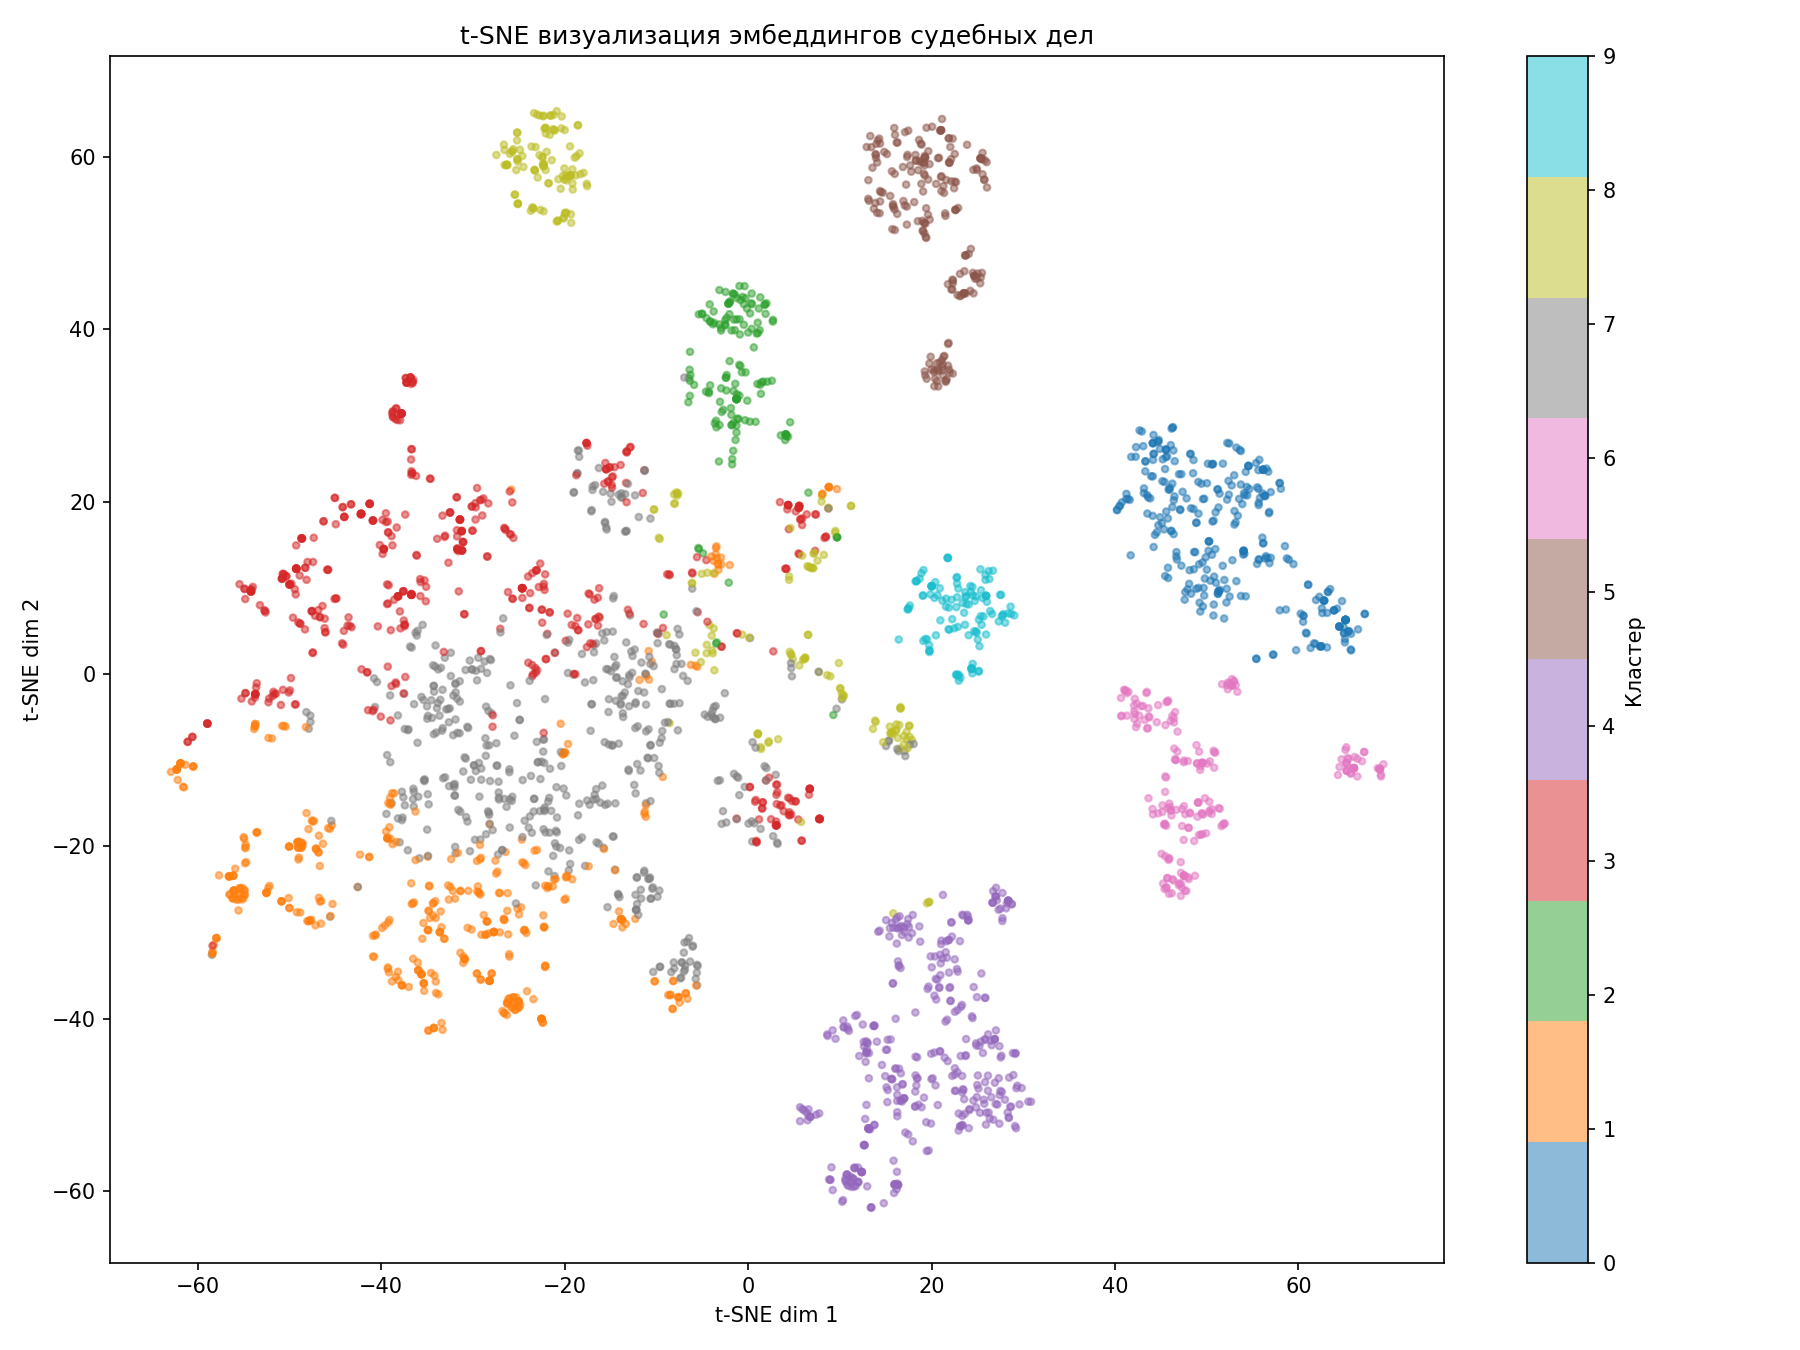
\includegraphics[width=\linewidth]{figures/embeddings_tsne.png}
  \caption{t-SNE projection of RuBERT-based case embeddings, with each point corresponding to a criminal court decision and colors indicating clusters in the embedding space.}
  \label{fig:tsne-embeddings}
\end{figure}

\begin{figure}[t]
  \centering
  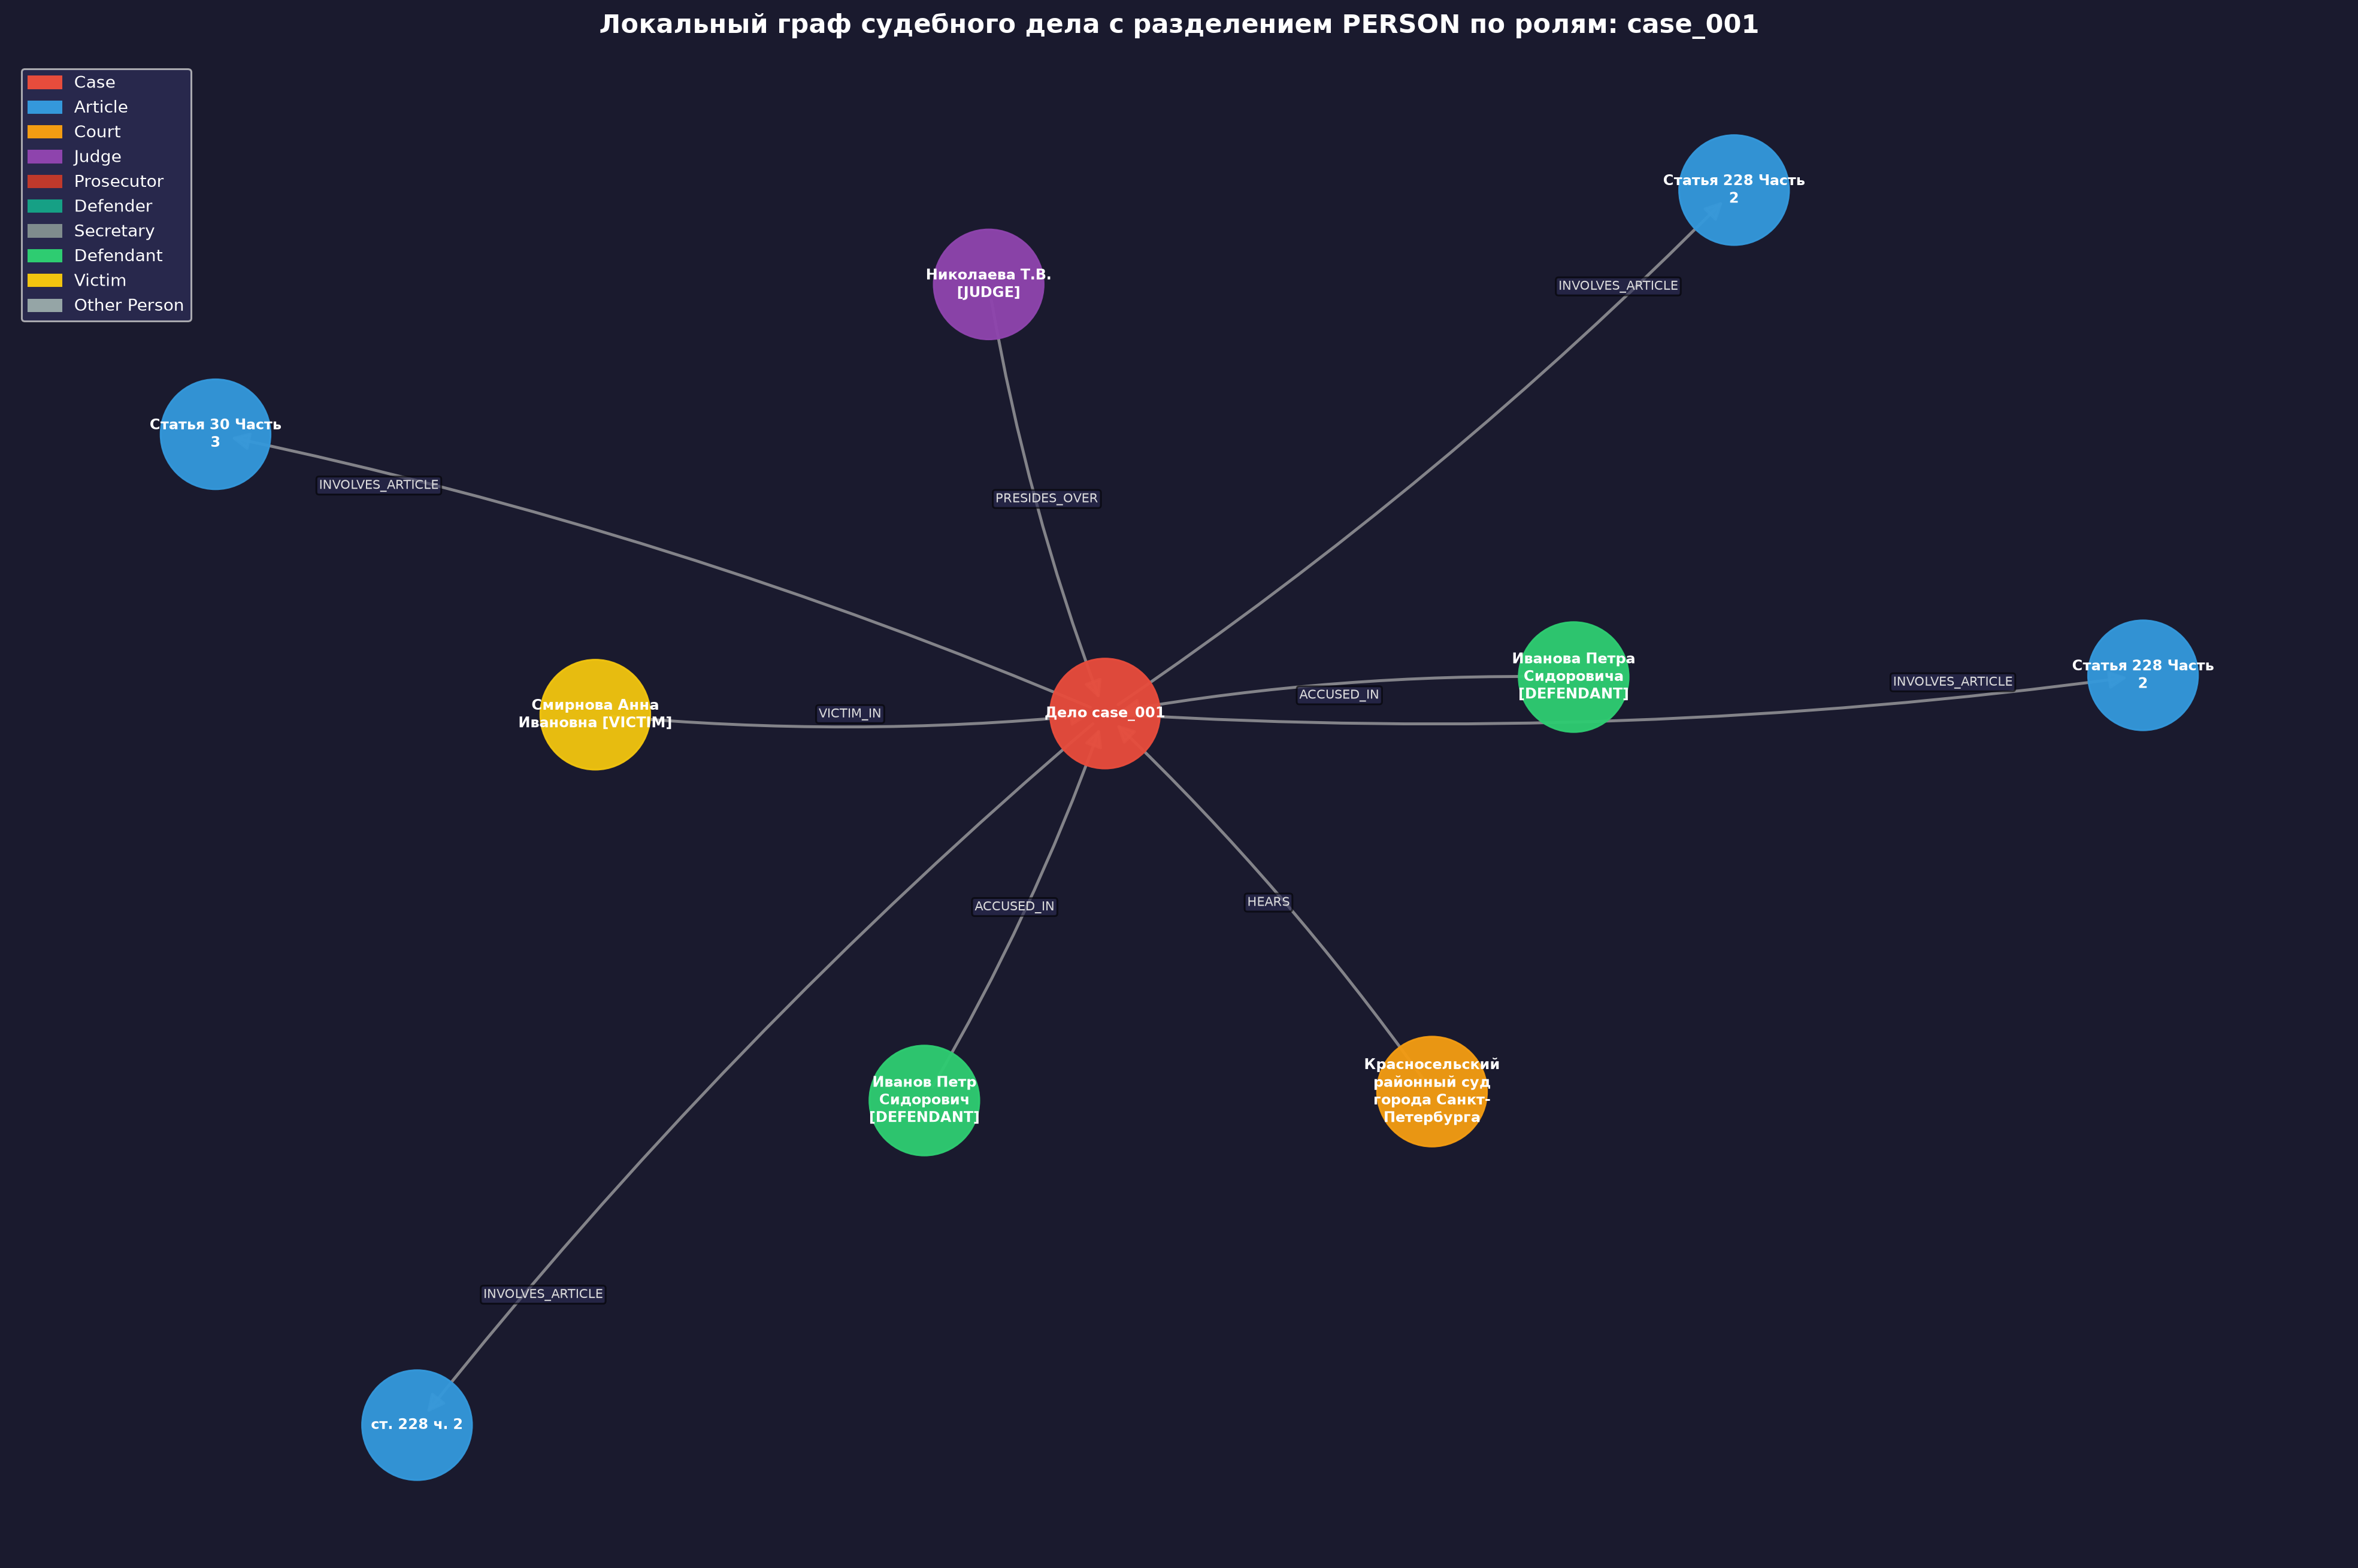
\includegraphics[width=\linewidth]{figures/demo_graph_roles_case_001.png}
  \caption{Local role-aware knowledge graph for a single criminal court case. The graph illustrates the extracted case, Criminal Code articles, court, and participants with their procedural roles (judge, defendant, victim), connected by semantic relations generated by the proposed information extraction pipeline.}
  \label{fig:streamlit-demo}
\end{figure}

Use cases for presentation and analysis include:
\begin{itemize}
\item \textbf{Article-based case navigation.} Given the global Neo4j graph, a Cypher query retrieves all cases involving a specified article (e.g., Article 228), along with their courts and regions, enabling a map-style overview of drug-related charges across the corpus.
\item \textbf{Judge exposure profiling.} A two-hop query finds judges who have presided over cases involving both Article 228 and Article 158, identifying courts where drug and theft offences are handled by the same bench.
\item \textbf{Defendant recidivism detection.} A degree query over \texttt{ACCUSED\_IN} edges identifies persons appearing as defendants in more than one case, subject to the limitations of name normalization noted below.
\item \textbf{Local case explanation.} For a selected case, the local subgraph provides a fully interpretable, human-readable summary: who was accused, under which articles, in which court, with which outcome. This is directly usable for supervisor presentations and conference demonstrations.
\end{itemize}

\section{Discussion}

\subsection{Strengths}

The rule-based approach to article extraction is transparent and reproducible and does not require labeled training data. Every pattern is human-readable, and each error can be traced back to a specific regex or normalization rule. The pattern inventory can be inspected, extended, and version-controlled in a straightforward way. The hybrid person NER pipeline achieves high recall---the property most critical for downstream graph completeness---at a modest false positive cost, and its combination of Natasha with regex fallback is simple to understand and maintain.

The role-aware graph schema supports a substantially richer query space than a flat participant-in-case model because each participant is explicitly connected to the case via an edge labeled with their procedural role. Users can ask not only ``who appears in this case?'' but also ``in what role?'' and traverse the graph along specific relations such as \texttt{PRESIDES\_OVER}, \texttt{ACCUSED\_IN}, or \texttt{VICTIM\_IN}. Figure~\ref{fig:streamlit-demo} illustrates a local role-aware knowledge graph for a single criminal court case: the \texttt{Case} node is linked to Criminal Code articles, the court, and participants with their assigned roles, making the structure of the decision visually interpretable and directly aligned with typical legal queries.

\subsection{Limitations}

The most significant limitation is that the graph currently represents \texttt{Article} nodes only at the article-number level, which means that the legally important distinction between Part~1 Art.~228 (simple possession) and Part~2 Art.~228 (possession with intent to distribute) is not preserved at the node level. This is an intentional simplification in the present schema, but it reduces the legal granularity of the graph. A future iteration may introduce separate nodes or attributes for parts and subparagraphs to capture these distinctions more faithfully.

A second limitation concerns morphological name normalization. Russian personal names inflect across grammatical cases, and the current pipeline may create distinct \texttt{Person} nodes for nominative and genitive forms of the same name. Full normalization via Natasha's \texttt{MorphVocab} module is planned but not yet implemented. This limitation has both analytic and ethical implications, since incorrect merging or splitting of person nodes can distort degree-based measures and aggregate counts.

A third limitation is the size and coverage of the evaluation data. The 20-case gold set, while carefully annotated, is small and may not represent the full diversity of citation forms and name formats present in the corpus. The evaluation therefore serves as a proof of concept rather than as a definitive benchmark. The error analysis suggests that certain edge cases, such as multi-article abbreviations, unusual punctuation, and rare name structures, remain undercovered.

\subsection{Perspectives and Future Positioning}

The system and evaluation framework address a research gap in Russian criminal court decisions and rule-based legal NLP for Cyrillic legal text, a setting that remains underrepresented in the NLLP literature. A submission to the NLLP workshop would naturally fit within the scope of legal NLP systems, legal knowledge graphs, and multilingual legal NLP, particularly given the workshop's emphasis in recent years on non-English and low-resource legal NLP settings. At the same time, the pipeline can serve as a baseline for future neural extensions that integrate RuBERT-based NER and classification models into the same graph architecture.

\section{Limitations and Ethical Considerations}

The case data used in this work originates from official Russian judicial portals, where court decisions are published in accordance with Russian legislation on judicial transparency. The personal names and facts processed by the pipeline are extracted from these publicly available documents exactly as they are published. Published decisions frequently appear in anonymized form, with personal names replaced by sequential placeholders (e.g., \texttt{Placeholder1}, \texttt{Placeholder2}) in accordance with data protection requirements for publicly released judicial records; no additional deanonymization has been performed.

The graph constructed by this pipeline is an exploratory research resource and must not be used as a source of certified legal information, as a basis for legal decisions, or as a tool for profiling individuals named in the cases. Aggregating cases into a graph can make certain patterns more salient than they are in individual decisions, for example the number of cases associated with a particular person node or the concentration of specific offences in a given region. Such aggregation can amplify existing biases in the underlying judicial data and must therefore be interpreted with caution.

The system does not perform any prediction of guilt, risk scoring, or outcome forecasting. All edges in the graph represent factual relations extracted from existing decisions (for example, ``Person~X was a defendant in Case~Y involving Article~228''). The pipeline is designed solely for search and analysis of already adjudicated cases and should not be used to inform decisions about individuals outside the context of those cases.

The three-regime evaluation framework reported in this paper shows that the reported performance depends substantially on the matching criterion that is applied. Readers should therefore attend carefully to the evaluation regime being cited when comparing results to other systems. In particular, the F1 score of 0.977 applies at the article-number level; at strict span-offset level, performance is substantially lower (F1 0.051), and the two figures are not interchangeable. Overstating the scope of high F1 scores would misrepresent the reliability of the system for tasks beyond article-number linkage.

The pipeline is designed for Russian criminal court decisions and would require substantial adaptation for other jurisdictions, legal systems, or languages. The regular expressions for article extraction are specific to the surface syntax of Russian Criminal Code citations and would not transfer to other legal codes without revision. The role-assignment patterns are tailored to Russian criminal procedure terminology and may misinterpret roles if applied to other domains. Furthermore, the person NER components may perform worse on uncommon names, foreign names, and multiple-surname structures; this has not been evaluated systematically and remains an open area for future work.

\section{Conclusion and Future Work}

This paper has presented a pipeline for constructing a legal knowledge graph over Russian criminal court decisions. Starting from raw JSON-encoded court files, the system applies rule-based NER for Criminal Code article references, a hybrid Natasha-plus-regex person NER module with role assignment for six procedural categories, and batch Cypher loading to Neo4j. The active demo graph currently contains 69{,}035 nodes and 399{,}551 relationships. The regex-based article extractor achieves precision 1.000, recall 0.955, and F1 0.977 at the article-number level on a manually annotated 20-case gold set, reflecting the deterministic and highly regular nature of Russian Criminal Code citation syntax. Person NER achieves an F1 score of 0.961 with perfect recall on 50 annotated mentions. The Streamlit-based demo interface exposes case search, local graph visualization, document-card inspection, and JSON export.

Future work encompasses several directions. On the extraction side, the regex article extractor will be extended to cover compound double-article abbreviated forms and subparagraph letter markers. Person name normalization will be improved using Natasha's \texttt{MorphVocab} inflected-form normalizer to collapse morphological variants of the same name into a single \texttt{Person} node. The type inventory will be extended to cover legal counsel, witnesses, and other participant roles as distinct node types, and verdict information will be lifted from a regex-based heuristic to a trained classifier that can handle more nuanced sentencing outcomes.

On the graph-analytics side, the embedding-based nearest-neighbour retrieval layer, currently stored as a separate RuBERT embedding CSV with precomputed cluster assignments, will be integrated into the demo interface to enable semantic case search alongside structural graph queries. The Cypher analytics suite will be extended to include multi-hop queries and Graph Data Science plugin operations such as PageRank and Louvain community detection over the full corpus graph. Finally, integration with citation graphs that connect cases referencing the same statutory provisions, or citing each other as precedents, represents a natural extension toward a richer legal knowledge graph that supports multi-layer legal analytics across statutes, cases, and participants.

\bibliographystyle{plain}
\bibliography{references}

\end{document}
